\renewcommand{\chaptername}{Chapter}
\chapter{Biological foundations: Prosodic deficits after a right-hemisphere brain stroke}\label{chap2}

%\jj{revoir l'organisation hiérarchique des sections (ex. deficits comme sous-partie de Stroke, puis deficits again en partie 2 etc.}

\section {Brain strokes: etiology, consequences and recovery}

\subsection{Etiology}

A stroke, or cerebrovascular accident, occurs when the brain's blood supply is disrupted, depriving it of oxygen and nutrients \jj{(REF)}. The \hl{most common} type of stroke is ischemic, caused by a blood clot blocking a vessel. Ischemic strokes include thrombotic strokes, where the clot forms in the clogged vessel, and embolic strokes, where the clot originates elsewhere (e.g., the heart) and travels to block brain arteries. \jj{say something about what effect ischemia has on neural cells and neural function}. \jj{The second type of stroke, } hemorrhagic, occurs when a weakened blood vessel ruptures, causing internal bleeding in the brain. The leaked blood \hl{puts pressure on nearby brain cells, leading to damage}.  \cite{kemmerer_cognitive_nodate}. Each year, an estimated 140,000 people in France are hospitalised for strokes \cite{lecoffre_laccident_nodate}. \jj{parler un peu de la mortalité?}.  Improved prognosis relies on prompt diagnosis and treatment during the acute phase after the onset of symptoms.

\subsection{Functional consequences} 

If a stroke damages critical brainstem regions essential for basic life functions, the individual may lose consciousness and die within minutes \jj{(REF)}. However, when the affected area is limited to cortical or white matter regions responsible for specific cognitive abilities, the person \jj{typically} survives but \jj{may} experiences deficits in those functions. For instance, strokes affecting the posterior cerebral artery, which supplies the occipital lobe \jj{(home to the visual cortices}), often lead to visual impairments. Similarly, strokes involving the middle cerebral artery, responsible for language-related perisylvian areas, typically result in linguistic deficits. \cite{kemmerer_cognitive_nodate}

\jj{More generally, and depending on its severity, surviving} a brain stroke is associated to a \hl{variety of physical and cognitive disabilities}, including \hl{muscle weakness}, \hl{perceptual disorders} such as aphasia \cite{hamilton_mechanisms_2011}, dementia \cite{leys_poststroke_2005}, and impairments in attention and memory \cite{lim_stroke_2009}. Some survivors may experience \hl{anosognosia} \cite{noauthor_anosognosia_nodate}, a condition where they are unaware of their own disabilities. \hl{Another common condition} is hemispatial neglect in which individuals are unable to attend to or perceive stimuli on the side of space opposite to the damaged \hl{hemisphere most frequently in the right cerebral hemisphere particularly in the acute stroke some of the manifestations} patients may exhibit repetitive, rhythmic movement disorders producing  perseverative behaviour of varying complexity \cite{ltd_spatial_2015}, additionally, 30–50\% of stroke survivors develop \hl{post-stroke depression} \cite{villain_facteurs_nodate}.

\subsection {Recovery after stroke} 
Rehabilitation after a stroke focuses on addressing the resulting deficits and \jj{the }challenges \jj{that come with them} \cite{licht_stroke_1975}. Physiotherapy and targeted exercises are often employed to restore physical movement \jj{(REF)}. Cognitive Behavioral Therapy (CBT) can be beneficial in managing anxiety, depression, and fatigue \cite{cumming_prevalence_2016} and \hl{enhance memory and concentration} which are common\jj{ly affected} after a stroke. \hl{Speech therapy} \cite{noauthor_speech_nodate} and specific exercises can address difficulties with speech, like functional communication, reading, writing, and expressive, receptive language. \jj{Is speech therapy a form of CBT ?}. \jj{In addition, a number of emerging} therapies and technological advancements \jj{are also proposed for} \st{are revolutionizing} stroke rehabilitation such as \hl{neuromodulation} \cite{saway_evolution_2024} or neurofeedback  \cite{wang_potential_2018}.\st{Speech therapy} \cite{noauthor_speech_nodate} \st{and specific exercises can address difficulties with speech, like functional communication, reading, writing, and expressive, receptive language}. 
 \jj{These approaches are often combined, and it is now widely recognized that} a multidisciplinary\jj{/multidomain recovery programs are best to} help stroke survivors regain independence and improve their quality of life \cite{langhorne_stroke_2011, benedetti_assessment_2022}.

\section{Language deficits}

The study of language has long been a topic of interest in psychology, but psycholinguistics as a distinct field only began to emerge in the 1960s, heavily influenced by Chomsky’s groundbreaking work in linguistics. Chomsky’s assertion that the unique properties of language require specialized cognitive mechanisms \cite{chomsky_linguistics_1991} provided the foundation for this field. 
\hl{Psycholinguistics initially focused on understanding language deficits} by investigating how different brain regions support language production and comprehension, advancing beyond a purely linguistic framework.

Aphasia, one of the most common language production deficits, is an impairment in the ability to produce, comprehend, or repeat language, typically resulting from damage to the left hemisphere. The National Aphasia Association estimates that 25–40 percent of stroke survivors develop aphasia \cite{kemmerer_cognitive_nodate}, with patients often struggling to retrieve words, form grammatically correct sentences, or understand phonemes, words, and syntax.

The first significant discoveries about the neural substrates of language arose from research on aphasia over 150 years ago. Two major types were identified: Broca's aphasia, associated with damage to the left inferior frontal gyrus, which impairs speech production and grammar, and Wernicke's aphasia, linked to damage in the superior temporal gyrus of the left hemisphere, resulting in deficits in the comprehension of written and spoken language.

Historically, the left hemisphere has been considered dominant for language processing, particularly in right-handed individuals. However, growing evidence highlights the right hemisphere's contributions to language function in neurologically normal individuals and its critical role in recovery following left-hemisphere brain damage \cite{kemmerer_cognitive_nodate}.

\section{Right Hemisphere stroke deficits} 
While much stroke research has centered on the left hemisphere, there is a growing acknowledgment of the subtle yet profound cognitive and communicative deficits that can arise from right hemisphere damage. Unlike aphasia as a well-recognized syndrome, which manifests in overt and easily identifiable by the Boston Diagnostic Aphasia Examination (BDAE), the challenges faced by individuals with right hemisphere damage are often less visible \cite{minga_apragmatism_2023}. These difficulties may only become evident through close interactions or observations by family members, who notice changes in their loved one’s ability to engage in meaningful spoken discourse, a monotone discourse and reduced participation in everyday communication.

Right hemisphere stroke leads to a range of communication and cognitive impairments that significantly impact the quality of life. 
Cognitive deficits lead individuals with RHD often to experience executive dysfunction, unilateral neglect and attention deficits are also common. Memory issues are frequently observed, including poor recall and working memory.
Approximately 96\% of adults with RHD in rehabilitation are impaired in at least one cognitive-communication domain \cite{blake_prevalence_2002}. ,\cite{tompkins_nature_2012}.

On the side of communication, deficits associated with RHD include linguistic challenges such as maintaining discourse coherence, selecting appropriate words, constructing syntactic structures, and managing conversational topics \cite{davis_referential_1997}. Impairments in the extralinguistic domain, such as difficulties in displaying appropriate emotional facial expressions and body language, further hinder effective communication. Paralinguistic deficits also play a significant role, with patients struggling to interpret and use non-literal language like idioms, metaphors, and sarcasm \cite{noauthor_spontaneous_nodate}. They may also have difficulty asking or understanding questions, exhibit tangential or egocentric discourse, and display verbosity or a paucity of speech. Furthermore, they often fail to grasp the main gist of conversations and suffer from aprosodia (difficulty in using or interpreting prosody), which is considered part of the pragmatic component of language \cite{stockbridge_aprosodia_2022, ukaegbe_aprosodia_2022}.

Recently, the term "apragmatism" has been proposed to describe the linguistic, paralinguistic, and extralinguistic deficits characteristic of right hemisphere damage (RHD). By adopting this label, to increase awareness of these pragmatic impairments, improve recognition, assessment, and treatment of these deficits within clinical and rehabilitative settings. \cite{minga_apragmatism_2023}


\subsection{Prosody} 
Prosody achieves what words alone often cannot—it shapes meaning, conveys emotions, and ensures the listener interprets the message correctly. In spoken communication, how something is said can be just as important as what is said. Often referred to as the "melody of language" \cite{hellerman_ann_2003}, \hl{prosody encompasses the song-like} vocal modulations that accompany speech, playing a crucial role in conveying emotions, structuring information, and distinguishing meanings. For instance, intonation can transform the statement "You finished writing the chapter." into the question "You finished writing the chapter?" Such subtle variations are indispensable for both linguistic and emotional communication, making prosody a fundamental element of speech.

Derived from the Greek word prosodia, meaning \hl{"sung to music,"} prosody refers to the suprasegmental features of speech at the word and sentence levels. It is defined by variations in acoustic parameters, including duration (measured in seconds), which reflects the rhythm of speech \cite{cummins_fascinating_2000}; sound intensity (measured in decibels), related to amplitude; and frequency of vocal fold vibration (measured in hertz), associated with pitch \cite{noauthor_theory_nodate}. Prosody conveys two functionally distinct yet interconnected categories of acoustic cues: emotional prosody and linguistic prosody. These cues—pitch, loudness, tempo(speech rate), and voice quality (timbre)—work together to enrich communication and ensure the intended message is understood. \aynaz{I'll add here music and prosody relation- pitch part}

\subsubsection{Emotional Prosody} 

Emotional prosody refers to the expressive and receptive modulation of intonation that \hl{conveys emotions} such as happiness, sadness, anger, and fear, as well as attitudes like sympathy, sarcasm, or dominance. It primarily relies on global changes in pitch height, loudness, and vocal rate, though other acoustic features also contribute to distinguishing emotional states. For instance, the phrase "John is leaving" can be expressed with a fast rate and high pitch to convey happiness or with a slow rate, low pitch, and reduced loudness to reflect sadness \cite{noauthor_good_nodate}(Kamiloğlu et al., 2020).

Affective prosody enables speakers to \hl{express emotions} and intentions while allowing listeners to interpret the emotional and attitudinal context of a message, thereby enriching verbal communication with depth and nuance. By providing emotional and social cues, it plays a crucial role in fostering effective interpersonal interactions \cite{sauter_cross-cultural_2010} \cite{ekman_pan-cultural_1969}.

\subsubsection{Linguistic Prosody} 
Linguistic prosody employs variations in tone, timing, and loudness to convey nuanced meanings in words and sentences. Its comprehension relies on the ability to perceive and integrate temporal and spectral variations, including phonemic and emphatic stress, syntactic boundaries, and phrasal groupings \cite{baum_sensitivity_2003}, \cite{ross_lateralization_1997}. Prosody plays a vital role in clarifying sentence structures, such as distinguishing between declarative and interrogative sentences. It also differentiates word meanings in tonal languages, where pitch variations can alter a word’s meaning, and emphasizes specific elements within a sentence to enhance understanding and communication \cite{ukaegbe_aprosodia_2022}.

\hl{For example}, prosodic cues distinguish between "White House" (the president's residence) and "white house" (a house that is white). Prosody also shapes intonation patterns, transforming sentences into questions through rising intonation or statements with falling intonation, often influenced by dialects and individual speech patterns. These melodic and rhythmic features of speech are indispensable for effective communication across various contexts and throughout different stages of life \cite{belyk_perception_2014}.

\subsubsection{Aprosodia}
Aprosodia, a condition characterized by difficulty in expressing or comprehending prosodic cues, stems from deficits in higher-level auditory processing during the attentive stage. These cues, which rely on suprasegmental features such as intonation, timing, pitch, amplitude, and stress\cite{ross_lateralization_1997}, \cite{gorelick_aprosodias_1987}, play a crucial role in conveying emotion, attitudes, and meaning. Aprosodia is estimated to affect 50\%–78\% of individuals with right hemisphere damage \cite{benton_right_1996} \cite{cancelliere_lesion_1990}\cite{cote_towards_2007}. \cite{ukaegbe_aprosodia_2022}

The pragmatic components of prosody can provide as much linguistic information as syntax or semantics, highlighting the importance of how something is said in shaping communication. For instance, a right hemisphere stroke patient may speak in a monotone pitch even when angry, making it difficult for listeners to discern their emotional state. Such deficits significantly hinder meaningful interpersonal interactions, impacting both linguistic and emotional communication \cite{gajardo-vidal_how_2018} \cite{sheppard_thats_2018}.

\subsubsection{Pitch}
Pitch is the basic and most general acoustic element of a spoken languagend serves as one of the primary auditory sensations essential for perceiving melody and harmony in music, as well as prosody in speech \cite{plack_pitch_2005}. Two critical aspects of pitch are first its relative height  which is reflective of the pitch level and the second one is the shape and direction of pitch (level, rising, dipping or falling) which is reflective of the pitch contour, The change of a pitch level is referred to as a step change in fundamental frequency (F0) from the sound onset (similar to music scales) whereas the change of a pitch contour is referred to as a consecutive change in F0 within tens to hundreds of milliseconds\cite{wang_hemispheric_2013}.

Pitch changes, such as detecting whether a sound is rising or falling in frequency pitch contours are processed as low-level features during early auditory processing. In contrast, later auditory processing handles high-level tasks, such as interpreting the meaning of an utterance and understanding its emotional context.

In non-tonal Indo-European languages like English and French, changes in pitch affect intonation rather than altering the meaning of words. Conversely, in tonal languages such as Mandarin Chinese, pitch plays a grammatical or lexical role, with variations in tone determining word meaning \cite{howie_acoustical_1976}. For instance, Mandarin has a four-tone system where the word "ma" can have four distinct meanings depending on its pitch. Notably, over 60\% of the world's languages are tonal.

\subsubsection{Lateralization of Prosody}
The lateralization of prosody is a critical topic in understanding how the brain processes both emotional and linguistic aspects of speech. Despite significant research, the division of prosody processing between the right hemisphere (RH) and left hemisphere (LH) remains a subject of debate, partly due to conflicting findings and the multifaceted nature of prosody. This complexity arises from variations in acoustic and functional features of prosody, as well as methodological differences in studies.

Several theories attempt to explain prosody lateralization and localization:
\begin{itemize}
\item \cite{blumstein_hemispheric_1974} suggested that the RH processes all prosodic features, while the LH focuses on segmental aspects.
\item Van Lancker (1980) \cite{noauthor_cerebral_nodate} proposed a functional distinction: the RH is specialized for affective prosody (e.g., emotional tones), and the LH for linguistic prosody (e.g., syntactic or lexical intonation).
\item \cite{behrens_characterizing_1989} posited that the RH processes global, sentence-level structures, while the LH handles local, syllable-level structures.
\item \cite{zatorre_lateralization_1992} demonstrated that pitch changes activate the RH prefrontal cortex, confirming its importance in pitch perception.
\item \cite{van_lancker_identification_1992} argued that lateralization depends on acoustic features, with the RH favoring pitch (F0) or long duration and the LH favoring temporal information or short duration, asymmetric sampling in time ; aligning with the dual-stream model of speech perception, where the RH specializes in slower, melodic changes, and the LH in rapid, temporal cues.\cite{zatorre_structure_2002}

\end{itemize}

Similarly, \cite{gandour_hemispheric_2004} emphasized that lateralization is influenced by language experience, which shapes the internal representation of prosodic elements. They highlighted a dynamic interaction between hemispheres via the corpus callosum, with the LH becoming more involved when language tasks extend beyond auditory analysis.

Moreover, a meta-analysis of functional neuroimaging showed that right posterior superior temporal gyrus (pSTG) was important for both emotional and linguistic prosody and also different prosodic functions are linked to different brain regions; mixed support for hemisphere lateralisation of speech prosody; lateralisation seen in temporal-lobe auditory areas more than in frontal-lobe evaluative areas; thereby promote a localizationist perspective. 
While affective prosody involves the IFG pars orbitalis, a region associated to limbic and speech-motor systems, linguistic prosody is linked to the IFG pars opercularis, which promotes syntactic processing, so acting as a critical interface between emotion and voice.  \cite{belyk_perception_2014}.

Sammler provided key insights into this topic using a novel paradigm combining audio morphing with multimodal neuroimaging and brain stimulation. They showed that prosody perception in the RH involves dual processing streams, similar to language processing in the LH. The dorsal pathway handles time-sensitive features ("how"), while the ventral pathway integrates these features into stable prosodic patterns ("what"). \cite{sammler_dorsal_2015}

\subsection{Related deficits}
Communication and cognitive impairments following a stroke often span multiple domains, from deficits in music perception and auditory attention to emotional regulation and perseverative behavior. Understanding the relationships between these impairments is essential for tailoring effective rehabilitation strategies. This section explores amusia, auditory processing, poststroke depression, and perseveration, shedding light on their interconnections and implications for stroke recovery.

\subsubsection{Amusia}
Traditionally, amusia and aphasia were considered dissociated deficits, reflecting the assumption of separate neural networks for music and speech perception. Recent research showing substantial overlap, particularly in processing speech prosody, such as intonation and emotional cues.
Aprosodia and amusia share a common neural foundation, involving damage to the right frontoinsular cortex, striatal regions, and disconnection of the right inferior fronto-occipital fasciculus. These impairments arise from disruptions in the right ventral auditory stream, which integrates rhythmic and melodic information essential for processing both prosody and music. This neural overlap complicates recovery and underscores the importance of targeted rehabilitation addressing impairments in both domains \cite{sihvonen_right_2022, hausen_music_2013}. The Montreal Battery of Evaluation of Amusia (MBEA) \cite{peretz_i_champod_as_and_hyde_k_varieties_2003} is a key tool for assessing music perception, focusing on melodic organization tasks such as scale, contour, and interval tests. By examining pitch perception—a shared feature of both amusia and aprosodia—the MBEA offers valuable insights for diagnosing and treating these interrelated deficits.
\subsubsection{Depression}
Neuropsychiatric disorders, particularly post-stroke depression (PSD), are frequent after stroke and have a profound impact on quality of life. A pilot study reported that 22.5\% of stroke patients developed PSD within the first three months following a stroke. Acoustic analysis revealed reduced variability in fundamental frequency along with significant alterations in voice breaks and shimmer, both of which were strong predictors of PSD risk. Early changes in affective prosody have been closely linked to an increased likelihood of developing PSD within the first period after stroke. \cite{villain_affective_2016}. 
\subsubsection{Perseveration}
Perseveration, characterized by repetitive behaviors or speech, is frequently observed in patients with spatial neglect following a stroke. Individuals with unilateral spatial neglect often fail to respond to stimuli on the contralesional side of space. In addition, they may exhibit perseverative behavior, such as repeatedly canceling stimuli on the ipsilesional side \cite{pia_drawing_2013}. This phenomenon is not merely a motor deficit but reflects broader cognitive impairments, including difficulties with attention, working memory, and executive functioning.

Attention, a complex cognitive function, is crucial for organizing and acquiring information that impacts behavior. Its role in perseverance is particularly significant, as deficits in sustained attention can lead to task abandonment or repetition of previous actions. The Logiciel d’Attention en Modalité Auditive (LAMA) is a validated tool designed to assess attentional abilities in the auditory modality. Originally developed to investigate the relationship between sensory aging and cognitive decline, LAMA evaluates sustained auditory attention and provides insights into how attentional deficits influence behavior \cite{ambert-dahan_capacites_2013}.

Studies, such as those using the Modern Cookie Theft picture description task, have highlighted the link between low conceptual units (CUs) and cognitive impairments in individuals with perseverative tendencies. These findings suggest that reduced speech output and early task abandonment may stem from attentional and memory deficits \cite{berube_analysis_2022}. However, despite these advances, the relationship between prosody and perseveration remains unexplored.

Another indirect impairment affecting prosody perception is the difficulty in discriminating sound intensity or duration. These auditory processing challenges can hinder an individual’s ability to perceive stress or rhythm in speech, which are critical components of prosody. Such impairments are often assessed using central auditory processing discrimination tasks for non-verbal sounds  Airtac2\cite{tessier_c_et_weill-chounlamountry_a_aide_2014}, highlighting their indirect but significant impact on prosody perception.
\subsubsection {Aprosody batteries}
Conscious awareness and education are key to ensuring that patients and their families understand the potential communication changes after a stroke. Speech language pathologists are trained to assess and treat cognitive-communication disorders, but patients are often not referred \cite{blake_prevalence_2002}, because these deficits can be hidden and hard to see in a brief clinic interaction. 
Although these deficits are subtle, comprehensive diagnostic batteries are essential for accurate identification and management. Commonly used batteries to diagnose prosody comprehensively evaluate patients' prosodic impairement.
Several diagnostic tools exist to assess prosody impairment, but they remain limited in scope and availability. Key tools include the Aprosodia Battery \cite{ross_lateralization_1997}, the Battery of Emotional Expression and Comprehension (BEEC;\cite{cancelliere_lesion_1990}), the New York Emotion Battery (NYEB;\cite{borod_j_welkowitz_j__obler_l_new_1992} ), the Montreal Protocol for the Evaluation of Communication (MEC; \cite{joanette_y_ska_b_et_ct_h_protocole_2004}), the Assessment Battery for Communication (ABaCo;\cite{angeleri_communicative_2008}) , the Affective Communication Test (ACT; \cite{friedman_understanding_1980}), Florida Affect Battery (FAB; \cite{walch_florida_1998}), and the Lille Communication Test (LCT; \cite{noauthor_communication_nodate}Rousseaux et al., 2010). 


Most tools focus primarily on emotional prosody, while linguistic prosody is underrepresented, appearing in subtests of five tools (FAB, MEC, ABaCo, NYEB, and LCT). Some tools also assess facial emotion perception and expression (e.g., BEEC, FAB, ACT, NYEB). Receptive prosody is challenging to evaluate due to the interpretive nature of emotional intent, while expressive prosody assessments are often influenced by subjective judgments of facial expressions and body language. Only three tools—EECB, Aprosodia Battery, and NYEB—focus on receptive skills.
Most tools are published in English, with only a few adapted for French (MEC, LCT) or Italian (ABaCo). \cite{benedetti_assessment_2022}

\subsection {MEC problems} 
\begin{figure}[ht!]
    \centering
    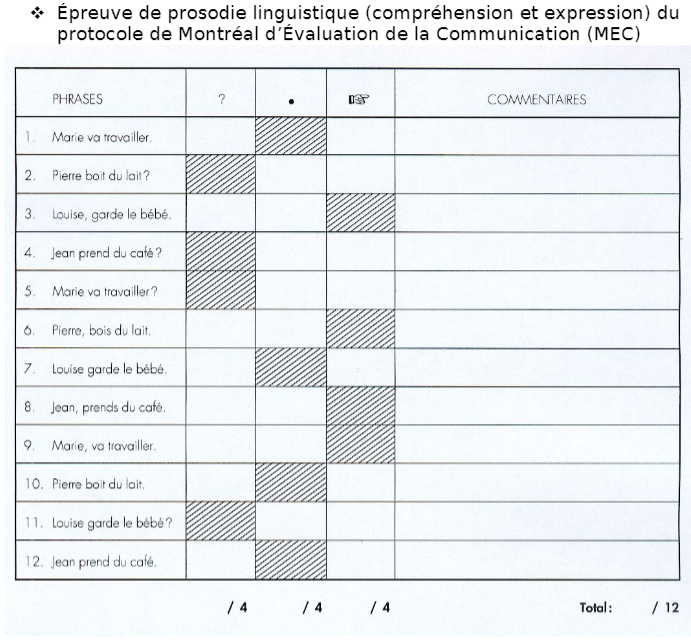
\includegraphics[width=6cm]{MainLayout/Images/chapter2/mec_c.png}
    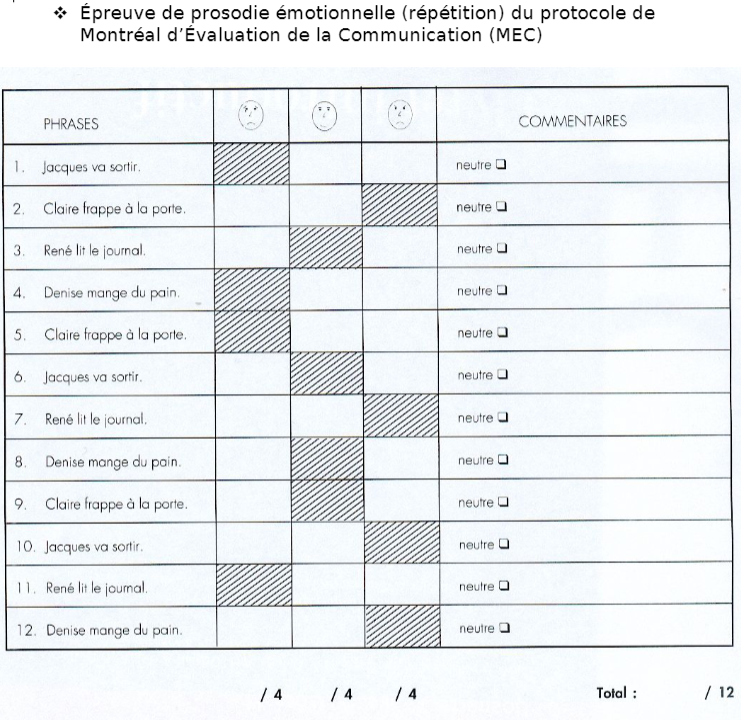
\includegraphics[width=6cm]{MainLayout/Images/chapter2/mec_r.png}
    \caption{Main Title for First Image \\ \small Subtitle for the first graphic.}
    \label{fig:mec_c}
\end{figure}  

Most of mentioned assessment tools above, including neuropsychological ("paper and pencil") tasks and functional assessments, aim to measure cognitive processes underlying prosodic abilities or evaluate real-life communication. However, these methods face considerable limitations. Manual scoring by clinicians often introduces inter-rater variability, and these tasks lack the sensitivity and replicability needed for accurately tracking therapy outcomes. For example, the Montreal Evaluation of Communication (MEC) \cite{joanette_y_ska_b_et_ct_h_protocole_2004}, widely regarded as the gold standard in French-speaking populations combines listening and production tests as shown in figure \ref{fig:mec_c} and \ref{fig:mec_r} , falls short in its "repetition task." This task, which requires patients to hear and reproduce a target expression, inadequately assesses perceptual representations or tests the ability to vocalize prosodic variations independently of auditory examples, limiting its diagnostic effectiveness.\cite{rosenbek_novel_2004}

A significant drawback of tools like the MEC is their susceptibility to test–retest effects. Participants may recall prior responses, leading to learning effects that undermine the reliability of results. Furthermore, most existing tools provide binary outcomes, simply indicating the presence or absence of a deficit. While such results can highlight pathology, they fail to explore the underlying mechanisms responsible for these deficits. \cite{benedetti_assessment_2022}

This broader lack of understanding of the sensory and cognitive mechanisms underlying aprosodia complicates accurate diagnosis and intervention. As a result, many prosodic deficits remain undetected, leaving patients at risk of inadequate treatment. This issue parallels the challenges observed in latent aphasia among left-hemisphere brain-damaged (LHBD) populations and the language deficits frequently associated with right-hemisphere brain damage (RHBD)\cite{martzoukou_undetected_2023}.


\section{Aim of the thesis}
The lack of sensitive tools for assessing prosody deficits has motivated this thesis to investigate the mechanisms underlying prosody perception. To address this challenge, we designed an innovative experiment that prioritizes practicality and efficiency. Instead of relying on traditional external reference-based approaches, our method encourages participants to evaluate stimuli based on their internal representations.

This design is tailored to the needs of stroke patients, minimizing fatigue and perseveration—two common challenges in this population, which are often compounded by attention loss and cognitive strain. By moving beyond conventional batteries, this experiment aims to not only enhance our theoretical understanding of prosody perception but also to create actionable insights for clinical practice. Ultimately, the framework developed here aspires to ensure that patients receive timely and targeted interventions for their specific deficits, addressing a critical gap in current diagnostic and treatment approaches.
